\documentclass[11pt,a4paper]{article}
\usepackage[T1]{fontenc}
\usepackage[utf8]{inputenc}
\usepackage{lmodern}
\usepackage[margin=2.5cm]{geometry}
\usepackage{amsmath,amssymb}
\usepackage{booktabs}
\usepackage{graphicx}
\usepackage{float}
\usepackage{caption}
\usepackage{enumitem}
\usepackage{microtype}
\usepackage{xcolor}
\usepackage[colorlinks=true,linkcolor=blue!50!black,urlcolor=blue!50!black,citecolor=blue!50!black]{hyperref}

\setlist{itemsep=2pt,topsep=4pt}
\emergencystretch=3em
\captionsetup{font=small,labelfont=bf}

\newcommand{\iu}{\mathrm{i}}
\newcommand{\code}[1]{\texttt{#1}}
\DeclareMathOperator{\Arg}{Arg}
\DeclareMathOperator{\wrap}{wrap}
\DeclareMathOperator{\E}{E}
\DeclareMathOperator{\RMSE}{RMSE}
\renewcommand{\Re}{\operatorname{Re}}
\renewcommand{\Im}{\operatorname{Im}}

\title{Experiment 1: point forecasts of wind with complex ARIMA}
\author{Wind Forecasting with Complex ARIMA --- working notes}
\date{30 September 2026 (runs 1--4)}

\begin{document}
\maketitle

\noindent All numbers below come from the scripts in \code{R/} and the tables in
\code{results/tables/}; the commands to reproduce them are in Section~\ref{sec:reproduce}.

\section{Aim}

The paper argues that wind should be modelled as \emph{one complex variable} (speed and direction
together) with complex ARIMA (cARIMA), rather than as two real series. Experiment~1 is the first
test of this: rolling-origin point forecasts of 10-minute wind, from 10 minutes to 6 hours ahead,
comparing cARIMA with persistence and with pairs of independent real ARIMA models.

\section{Data}

\begin{itemize}
  \item Kaggle Wind Turbine SCADA dataset, file \code{T1.csv}: one turbine in Turkey, 2018,
    10-minute resolution, wind speed (m/s) and wind direction (degrees). Details are in
    \code{data/README.md}.
  \item 50,530 rows on a 52,560-slot grid: 2,030 missing slots, including three gaps longer than
    3 days.
  \item \code{R/02\_prepare\_data.R}:
  \begin{itemize}
    \item puts the data on a regular 10-minute grid;
    \item fills gaps of at most 36 slots (6 hours) by linear interpolation of $\Re Z_t$ and
      $\Im Z_t$ (defined below);
    \item replaces speeds below 0.1\,m/s (10 exact zeros) by 0.1, so that logarithms exist;
    \item treats an origin as \emph{eligible} if its 4-week training window has no missing values,
      and its 6-hour horizon has no missing values and no values from interpolations longer than
      3 slots.
  \end{itemize}
  \item The first eligible window (2018-01-30 14:40 to 2018-02-27 14:30) is the \emph{selection
    window}. The 300 test origins are spread evenly over the later eligible origins (2018-02-27
    14:40 to 2018-12-31 17:50; none in October, because of gaps).
\end{itemize}

\section{How the wind is modelled}

\subsection{Wind as a complex number}

With speed $v_t > 0$ and direction angle $\theta_t \in (-\pi, \pi]$, the wind is
\begin{equation}
  Z_t = v_t e^{\iu\theta_t} = v_t\cos\theta_t + \iu\, v_t\sin\theta_t .
\end{equation}
$\Re Z_t$ and $\Im Z_t$ are the plain Cartesian coordinates of the wind vector (not the
meteorological zonal and meridional components).

\subsection{Complex ARIMA}

The cARIMA$(p,d,q)$ model is the ARIMA model with the variable and all parameters complex:
\begin{equation}\label{eq:carima}
  \Bigl(1 - \sum_{j=1}^{p}\phi_j B^j\Bigr)(1-B)^d\, y_t
  = \beta_0 + \Bigl(1 + \sum_{j=1}^{q}\theta_j B^j\Bigr)\varepsilon_t,
  \qquad \phi_j, \theta_j, \beta_0 \in \mathbb{C},
\end{equation}
where $B$ is the backshift operator. It is estimated by maximum likelihood with
\code{complex::clm()}; in run~4 the orders are selected with \code{complex::auto.carima()}.

Multiplying by a complex coefficient $\phi = a + \iu b = r e^{\iu\alpha}$ \emph{scales} by $r$ and
\emph{rotates} by $\alpha$. Written for the pair $(\Re y, \Im y)$,
\begin{equation}
  \begin{pmatrix} \Re(\phi y) \\ \Im(\phi y) \end{pmatrix}
  = \begin{pmatrix} a & -b \\ b & a \end{pmatrix}
    \begin{pmatrix} \Re y \\ \Im y \end{pmatrix},
\end{equation}
so cARIMA is a restricted bivariate VARIMA with 2 real parameters per lag instead of 4. This
parsimony relative to VAR is the central argument of the paper.

The error $\varepsilon_t$ is complex normal with variance $\sigma^2 = \E|\varepsilon_t|^2$ and
pseudo-variance $\tau = \E\varepsilon_t^2$ (for zero-mean errors). In terms of the real and
imaginary parts,
\begin{equation}
  \operatorname{Var}(\Re\varepsilon_t) = \tfrac12(\sigma^2 + \Re\tau), \quad
  \operatorname{Var}(\Im\varepsilon_t) = \tfrac12(\sigma^2 - \Re\tau), \quad
  \operatorname{Cov}(\Re\varepsilon_t, \Im\varepsilon_t) = \tfrac12\Im\tau .
\end{equation}
If $\tau \neq 0$ the error is \emph{non-circular}: its scatter is an ellipse rather than a circle.
For wind this is anisotropy, a prevailing direction of change. We summarise it by the index
\begin{equation}\label{eq:noncirc}
  \kappa = \frac{|\tau|}{\sigma^2} \in [0, 1],
\end{equation}
which is 0 for circular errors and 1 for errors lying on a line.

\subsection{Why logarithms}

The main target is the complex logarithm
\begin{equation}
  \log Z_t = \log v_t + \iu\,\tilde\theta_t ,
\end{equation}
where $\tilde\theta_t$ is the unwrapped angle (Section~\ref{sec:diff}).
\begin{itemize}
  \item It \emph{separates speed and direction}: the real part is log speed, the imaginary part is
    the angle. A cARIMA on $\log Z_t$ is still one complex model: the two parts are linked
    through the complex coefficients and the error covariance.
  \item Changes of speed are roughly \emph{multiplicative}: they are larger when it is windy, so
    log speed is a more natural scale than speed.
  \item The back-transform $\hat Z_{t+h} = \exp(\widehat{\log Z}_{t+h})$ always gives a positive
    speed and a valid angle.
  \item $\exp(\widehat{\log Z}_{t+h})$ is not the conditional mean of $Z_{t+h}$. This experiment
    does not correct for that.
\end{itemize}
The models on $Z_t$ itself are kept for comparison.

\subsection{Why differences, and angle unwrapping}\label{sec:diff}

\begin{itemize}
  \item 10-minute wind is very persistent: over a 4-week window the level wanders without a
    stable mean, and persistence is a hard benchmark. So in runs 1--3 all models use $d = 1$. With
    logarithms the differences have a clear meaning:
    \begin{equation}
      (1-B)\log Z_t = \log\frac{v_t}{v_{t-1}} + \iu\,(\tilde\theta_t - \tilde\theta_{t-1}),
    \end{equation}
    the log ratio of speeds and the change of direction.
  \item The angle in $(-\pi, \pi]$ jumps by about $2\pi$ whenever the wind crosses the cut (696
    times in \code{T1.csv}). In the differences these would be huge artificial shocks. Therefore,
    within each training window $t = 1, \dots, T$, the angle is unwrapped:
    \begin{equation}
      \tilde\theta_1 = \theta_1, \qquad
      \tilde\theta_t = \tilde\theta_{t-1} + \wrap(\theta_t - \theta_{t-1}), \qquad
      \wrap(x) = \operatorname{atan2}(\sin x, \cos x),
    \end{equation}
    so that $\tilde\theta_t - \tilde\theta_{t-1}$ is the shortest-arc change. Forecasts are
    wrapped back to $(-\pi, \pi]$ for evaluation.
  \item \code{clm()} estimates the model in the ``direct'' form: forecasts are produced in levels,
    and models with different $d$ are comparable by information criteria.
  \item In run~4, \code{auto.carima()} may choose $d \in \{0, 1\}$. It picks $d = 0$ for $Z_t$,
    with $\phi_1 \approx 0.993$--$0.994$. The half-life of a deviation from the mean,
    $\log 0.5 / \log|\phi_1|$, is about 100--120 steps, i.e.\ 16--20 hours. For $\log Z_t$ it picks
    $d = 1$.
\end{itemize}

\begin{figure}[H]
  \centering
  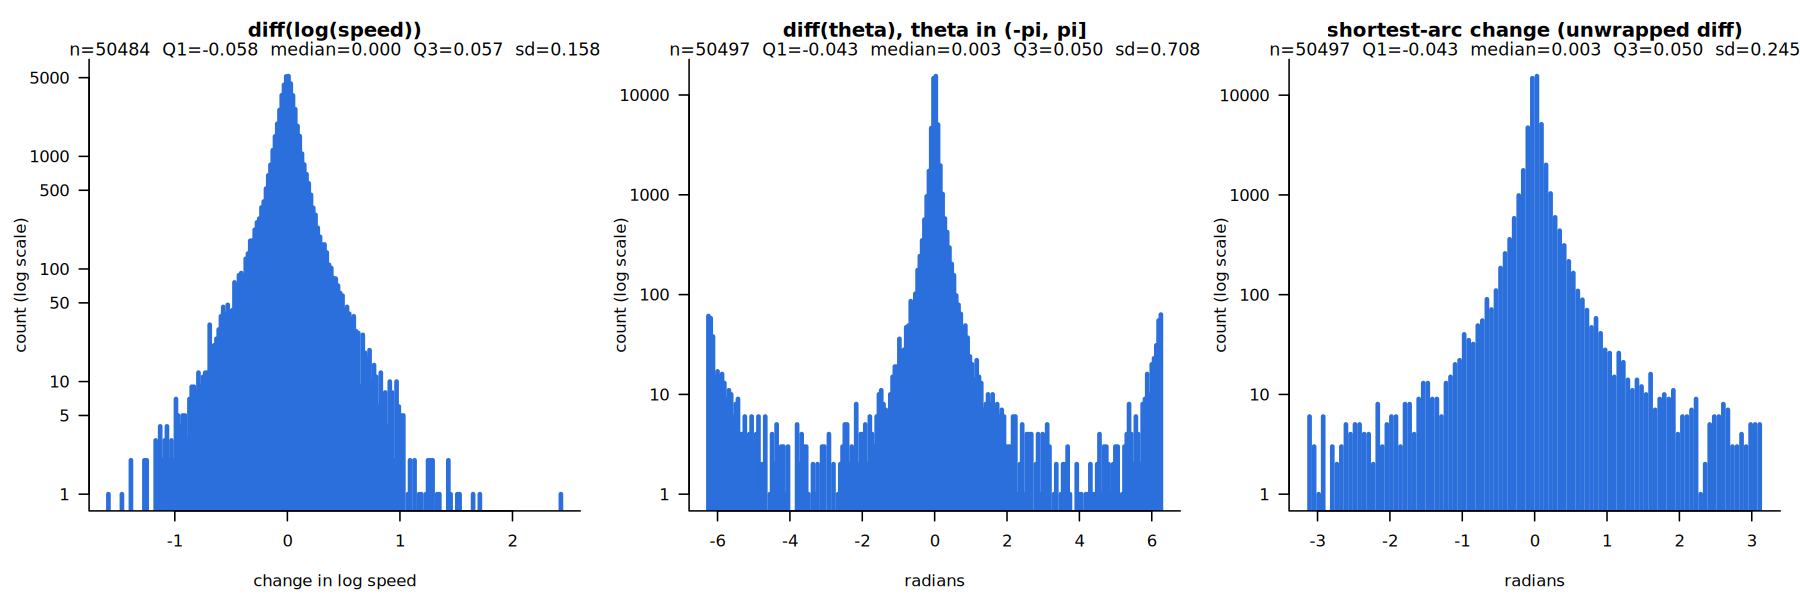
\includegraphics[width=\textwidth]{../figures/diffs_hist.png}
  \caption{10-minute changes in \code{T1.csv} (log-scale counts): log speed; the wrapped angle
    difference, with its $\pm 2\pi$ jumps; and the shortest-arc angle change.}
\end{figure}

\subsection{Why the complex generalised normal distribution}

The 10-minute changes have very heavy tails. Table~\ref{tab:kurt} gives the kurtosis
$\E(x - \E x)^4 / (\operatorname{Var} x)^2$ of consecutive changes in \code{T1.csv}; it is 3 for
a normal distribution. About 3\% of angle changes exceed $30^\circ$ and 0.5\% exceed $90^\circ$.

\begin{table}[H]
  \centering
  \caption{Kurtosis of 10-minute changes (normal: 3).}\label{tab:kurt}
  \begin{tabular}{lr}
    \toprule
    change & kurtosis \\
    \midrule
    $\log v_t - \log v_{t-1}$ & 14.4 \\
    $\wrap(\theta_t - \theta_{t-1})$ & 52.8 \\
    $\Re Z_t - \Re Z_{t-1}$ & 131.9 \\
    $\Im Z_t - \Im Z_{t-1}$ & 25.5 \\
    \bottomrule
  \end{tabular}
\end{table}

Under a normal likelihood these outliers pull the estimates, in particular the constant. For
$\log Z_t$ with $d = 1$, $\Im\beta_0$ is a steady rotation of the forecasts: $0.0122$\,rad
($0.70^\circ$) per step in \code{carima\_logZ}, i.e.\ about $25^\circ$ over the 6-hour horizon.
(The project notes for run~2 record a median rotation of $17^\circ$ at $h = 36$ for the normal model
and $5^\circ$ with the generalised normal; this was not recomputed here.)

We therefore also use the complex generalised normal distribution (\code{distribution = "dcgnorm"}
in \code{clm()}; Novey, Adali and Roy, 2010). For the error $e = z - \mu$, with scale $\alpha^2$,
pseudo-scale $\psi^2$ and shape $\beta$,
\begin{equation}\label{eq:cgnorm}
  f(z) = \frac{2\beta}{\pi\,\Gamma(1/\beta)\, 2^{1/\beta}\sqrt{\alpha^4 - |\psi^2|^2}}
         \exp\Bigl(-\tfrac12 Q^\beta\Bigr),
  \qquad
  Q = \frac{2\bigl(\alpha^2|e|^2 - \Re(\overline{\psi^2}\, e^2)\bigr)}{\alpha^4 - |\psi^2|^2}.
\end{equation}
For $\beta = 1$ this is the complex normal distribution with variance $\alpha^2$ and pseudo-variance
$\psi^2$; $\beta < 1$ gives heavier tails ($\beta = 0.5$ is Laplace-like). The variance and
pseudo-variance are $\alpha^2$ and $\psi^2$ multiplied by $2^{1/\beta}\Gamma(2/\beta) /
(2\Gamma(1/\beta))$. The shape is estimated, while the scale and pseudo-scale are concentrated out in
closed form. The estimates are $\hat\beta \approx 0.21$ for $\log Z_t$ and $\hat\beta \approx 0.41$
for $Z_t$, far from normal. On the selection window the generalised normal raises the
log-likelihood by about 5,000 ($\log Z_t$) and 1,500 ($Z_t$).

\section{Experimental design}

The pipeline is \code{R/02\_prepare\_data.R} $\to$ \code{R/03\_select\_orders.R} $\to$
\code{R/04\_rolling\_origin.R} $\to$ \code{R/05\_evaluate.R}. Shared code is in
\code{R/functions.R}, and the parameter tables come from \code{R/06\_parameters.R}.

\begin{itemize}
  \item \textbf{Rolling origin:} 300 origins, a window of 4 weeks ($T = 4032$ observations),
    horizons $h = 1, \dots, 36$ (10 minutes to 6 hours). Parameters are re-estimated at every
    origin.
  \item \textbf{Order selection} is done once, on the selection window; the orders are then fixed
    for all origins.
  \begin{itemize}
    \item cARIMA, runs 1--3: $d = 1$, and $p, q \in \{0, \dots, 3\}$ by AICc. From its default start,
      \code{clm()} can end in a poor local optimum, so each fit also starts from the estimates of
      the nested models $(p-1, q)$ and $(p, q-1)$ and keeps the highest log-likelihood.
    \item cARIMA, run 4: stepwise search with
      \[\text{\code{auto.carima(y, orders = list(ar = 3, i = 1, ma = 3), constant = NULL)}},\]
      which chooses $p, q \le 3$, $d \le 1$ and whether to include $\beta_0$.
    \item Real benchmarks: \code{forecast::auto.arima} with $d = 1$; \code{smooth::auto.msarima}
      on the differenced series, then refitted with $d = 1$.
    \item At each origin, cARIMA fits start from the default and from the selection-window
      estimates.
  \end{itemize}
  \item \textbf{Error measures}, in original units, for origin $t$ and horizon $h$:
    \begin{align}
      e^{\text{speed}}_{t,h} &= |\hat Z_{t+h|t}| - |Z_{t+h}| \quad \text{(m/s)}, \\
      e^{\text{angle}}_{t,h} &= \tfrac{180}{\pi}\wrap\bigl(\Arg\hat Z_{t+h|t} - \Arg Z_{t+h}\bigr)
        \quad \text{(degrees)}, \\
      e^{\text{vector}}_{t,h} &= |\hat Z_{t+h|t} - Z_{t+h}| \quad \text{(m/s)},
    \end{align}
    and $\RMSE_h = \bigl(\frac{1}{300}\sum_t e_{t,h}^2\bigr)^{1/2}$. The column ``h1--36'' pools all
    horizons.
\end{itemize}

\begin{table}[H]
  \centering
  \caption{Models. The real benchmarks forecast two series independently and combine them into
    $\hat Z$: (speed, angle), (log speed, angle) and $(\Re Z, \Im Z)$. Run~1: cARIMA with a constant
    and the real benchmarks; run~2: generalised normal; run~3: $\log Z$ without a constant
    (\code{\_nd}); run~4: \code{auto.carima}.}\label{tab:models}
  \resizebox{\textwidth}{!}{%
  \begin{tabular}{lllll}
    \toprule
    model & series & distribution & orders & constant $\beta_0$ \\
    \midrule
    \code{persistence} & -- & -- & $\hat Z_{t+h|t} = Z_t$ & -- \\
    \midrule
    \code{carima\_logZ} & $\log Z$ & normal & $d = 1$, AICc & yes \\
    \code{carima\_logZ\_cgn} & $\log Z$ & generalised normal & $d = 1$, AICc & yes \\
    \code{carima\_logZ\_nd} & $\log Z$ & normal & $d = 1$, AICc & no \\
    \code{carima\_logZ\_cgn\_nd} & $\log Z$ & generalised normal & $d = 1$, AICc & no \\
    \code{carima\_z} & $Z$ & normal & $d = 1$, AICc & yes \\
    \code{carima\_z\_cgn} & $Z$ & generalised normal & $d = 1$, AICc & yes \\
    \midrule
    \code{auto\_carima\_logZ} & $\log Z$ & normal & \code{auto.carima} & selected \\
    \code{auto\_carima\_logZ\_cgn} & $\log Z$ & generalised normal & \code{auto.carima} & selected \\
    \code{auto\_carima\_z} & $Z$ & normal & \code{auto.carima} & selected \\
    \code{auto\_carima\_z\_cgn} & $Z$ & generalised normal & \code{auto.carima} & selected \\
    \midrule
    \code{arima\_*}, \code{msarima\_*} & two real series & normal &
      \code{auto.arima} / \code{auto.msarima}, $d = 1$ & selected \\
    \bottomrule
  \end{tabular}}
\end{table}

\section{Selected orders and estimated parameters}

Table~\ref{tab:params} gives the estimates on the selection window
(\code{results/tables/parameters\_carima.csv}); in the rolling origin they are re-estimated at
every origin. The coefficients follow the signs in \eqref{eq:carima}. Standard errors are not
reported: \code{summary()} fails on these fits in the current package version (its \code{vcov}
refit cannot find \code{distribution}).

\begin{table}[H]
  \centering
  \caption{cARIMA estimates on the selection window. $\hat\beta$ is the shape of the generalised
    normal.}\label{tab:params}
  \resizebox{\textwidth}{!}{%
  \begin{tabular}{llllllr}
    \toprule
    model & $(p,d,q)$ & $\hat\beta_0$ & $\hat\phi_1$ & $\hat\theta_1, \dots, \hat\theta_q$ & $\hat\beta$ &
      log-likelihood \\
    \midrule
\texttt{carima\_logZ} & (0,1,3) & $-0.0003+0.0122\mathrm{i}$ & -- & \begin{tabular}[t]{@{}l@{}}$-0.0856-0.0148\mathrm{i}$ \\ $-0.0511-0.0018\mathrm{i}$ \\ $-0.0250+0.0011\mathrm{i}$\end{tabular} & -- & $493.33$ \\
\texttt{carima\_logZ\_cgn} & (0,1,2) & $0.0001+0.0012\mathrm{i}$ & -- & \begin{tabular}[t]{@{}l@{}}$0.0607+0.0056\mathrm{i}$ \\ $-0.0649+0.0047\mathrm{i}$\end{tabular} & 0.212 & $5510.52$ \\
\texttt{carima\_z} & (0,1,2) & $-0.0026-0.0005\mathrm{i}$ & -- & \begin{tabular}[t]{@{}l@{}}$-0.0281-0.0245\mathrm{i}$ \\ $-0.1250+0.0375\mathrm{i}$\end{tabular} & -- & $-9906.10$ \\
\texttt{carima\_z\_cgn} & (0,1,2) & $-0.0016+0.0088\mathrm{i}$ & -- & \begin{tabular}[t]{@{}l@{}}$0.0306+0.0023\mathrm{i}$ \\ $-0.1000+0.0250\mathrm{i}$\end{tabular} & 0.408 & $-8420.80$ \\
\texttt{carima\_logZ\_nd} & (1,1,2) & none & $0.6264-0.0111\mathrm{i}$ & \begin{tabular}[t]{@{}l@{}}$-0.7074+0.0000\mathrm{i}$ \\ $0.0000+0.0000\mathrm{i}$\end{tabular} & -- & $492.51$ \\
\texttt{carima\_logZ\_cgn\_nd} & (0,1,2) & none & -- & \begin{tabular}[t]{@{}l@{}}$0.0650+0.0089\mathrm{i}$ \\ $-0.0774+0.0131\mathrm{i}$\end{tabular} & 0.212 & $5509.75$ \\
\texttt{auto\_carima\_z} & (1,0,2) & $-0.0159+0.0138\mathrm{i}$ & $0.9930+0.0022\mathrm{i}$ & \begin{tabular}[t]{@{}l@{}}$-0.0270-0.0287\mathrm{i}$ \\ $-0.1293+0.0394\mathrm{i}$\end{tabular} & -- & $-9888.61$ \\
\texttt{auto\_carima\_z\_cgn} & (1,0,2) & $-0.0102+0.0212\mathrm{i}$ & $0.9943+0.0006\mathrm{i}$ & \begin{tabular}[t]{@{}l@{}}$0.0344+0.0010\mathrm{i}$ \\ $-0.0918+0.0197\mathrm{i}$\end{tabular} & 0.409 & $-8408.73$ \\
\texttt{auto\_carima\_logZ} & (1,1,1) & $0.0000+0.0044\mathrm{i}$ & $0.6427+0.0044\mathrm{i}$ & \begin{tabular}[t]{@{}l@{}}$-0.7250-0.0145\mathrm{i}$\end{tabular} & -- & $499.72$ \\
\texttt{auto\_carima\_logZ\_cgn} & (0,1,2) & none & -- & \begin{tabular}[t]{@{}l@{}}$0.0685+0.0017\mathrm{i}$ \\ $-0.0710+0.0003\mathrm{i}$\end{tabular} & 0.213 & $5509.95$ \\
    \bottomrule
  \end{tabular}}
\end{table}

\begin{itemize}
  \item \textbf{Constants.} For $\log Z_t$, $\Im\hat\beta_0$ is the angle drift per 10 minutes:
    $0.0122$\,rad for \code{carima\_logZ}, the same as the drift of the real \code{arima\_angle}
    model ($0.0121$, Table~\ref{tab:bench}). The generalised normal shrinks it to $0.0012$.
    \code{auto.carima} keeps the constant for $\log Z_t$ with the normal distribution and drops it
    with the generalised normal.
  \item \textbf{$Z_t$ with $d = 0$.} $\hat\phi_1$ is close to 1 with an almost zero argument:
    close to a unit root, without rotation. The implied long-run mean
    $\mu = \beta_0/(1 - \phi_1)$ is $-2.63 + 1.14\iu$ (normal) and $-2.16 + 3.49\iu$ (generalised
    normal), vectors of 2.9 and 4.1\,m/s. For comparison, the mean \emph{speed} in the window is
    8.5\,m/s, but the mean \emph{vector} is only 3.5\,m/s long, because winds from different
    directions cancel out. Reverting to the mean therefore shrinks $|\hat Z|$ at long horizons.
  \item \code{auto\_carima\_logZ\_cgn} selected $(0,1,2)$ without a constant, the same
    specification as \code{carima\_logZ\_cgn\_nd}.
  \item \textbf{Caveat, \code{carima\_logZ\_nd}.} Refitting $(1,1,2)$ reaches a log-likelihood
    of $492.51$, above the $489.91$ found during order selection
    (\code{carima\_order\_grid.csv}). The best fit has $\hat\theta_2 = 0$ exactly, which suggests
    the optimiser stayed at the starting values padded from the nested $(1,1,1)$ model. So the
    order selection for this model used a sub-optimal fit, and $(1,1,1)$ may have been the better
    choice. All other models reproduce the selection log-likelihood to within 0.02.
\end{itemize}

Table~\ref{tab:resid} gives the sample covariance of the residuals $(\Re\hat\varepsilon_t,
\Im\hat\varepsilon_t)$ and the non-circularity index \eqref{eq:noncirc}, computed from the
centred residuals $\tilde\varepsilon_t = \hat\varepsilon_t - \frac1T\sum_s\hat\varepsilon_s$ as
$\hat\kappa = \bigl|\sum_t\tilde\varepsilon_t^2\bigr| / \sum_t|\tilde\varepsilon_t|^2$.
Values of $0.27$--$0.33$ mean clearly elliptical errors, i.e.\ a prevailing direction of change,
which a pair of independent real models ignores.

\begin{table}[H]
  \centering
  \caption{Residuals on the selection window: standard deviations and correlation of the real and
    imaginary parts, and the non-circularity $\kappa$.}\label{tab:resid}
  \begin{tabular}{lrrrr}
    \toprule
    model & sd $\Re\hat\varepsilon$ & sd $\Im\hat\varepsilon$ & $\operatorname{cor}(\Re\hat\varepsilon,
      \Im\hat\varepsilon)$ & $\kappa$ \\
    \midrule
\texttt{carima\_logZ} & 0.196 & 0.265 & $-0.076$ & 0.304 \\
\texttt{carima\_logZ\_cgn} & 0.201 & 0.264 & $-0.054$ & 0.271 \\
\texttt{carima\_z} & 0.901 & 0.798 & $0.310$ & 0.330 \\
\texttt{carima\_z\_cgn} & 0.904 & 0.800 & $0.311$ & 0.332 \\
\texttt{carima\_logZ\_nd} & 0.195 & 0.265 & $-0.075$ & 0.306 \\
\texttt{carima\_logZ\_cgn\_nd} & 0.201 & 0.264 & $-0.051$ & 0.269 \\
\texttt{auto\_carima\_z} & 0.900 & 0.796 & $0.310$ & 0.331 \\
\texttt{auto\_carima\_z\_cgn} & 0.903 & 0.799 & $0.313$ & 0.334 \\
\texttt{auto\_carima\_logZ} & 0.195 & 0.266 & $-0.075$ & 0.306 \\
\texttt{auto\_carima\_logZ\_cgn} & 0.201 & 0.264 & $-0.053$ & 0.269 \\
    \bottomrule
  \end{tabular}
\end{table}

\begin{table}[H]
  \centering
  \caption{Real benchmarks on the selection window (\code{results/tables/parameters\_benchmarks.csv}).
    $\phi_j$: AR, $\theta_j$: MA (sign convention $1 + \theta_1 B + \dots$), $c$: drift.}
    \label{tab:bench}
  \resizebox{\textwidth}{!}{%
  \begin{tabular}{lllp{10.5cm}}
    \toprule
    model & $(p,d,q)$ & drift & coefficients \\
    \midrule
\texttt{arima\_speed} & (5,1,3) & no & $\phi_{1}=-0.5156$, $\phi_{2}=0.1343$, $\phi_{3}=0.7397$, $\phi_{4}=0.0330$, $\phi_{5}=0.0443$, $\theta_{1}=0.4364$, $\theta_{2}=-0.2834$, $\theta_{3}=-0.7965$ \\
\texttt{msarima\_speed} & (3,1,2) & yes & $\phi_{1}=0.3978$, $\phi_{2}=0.2726$, $\phi_{3}=0.0589$, $\theta_{1}=-0.4786$, $\theta_{2}=-0.3482$, $c=-0.0002$ \\
\texttt{arima\_logSpeed} & (1,1,2) & no & $\phi_{1}=0.7313$, $\theta_{1}=-0.9495$, $\theta_{2}=0.0767$ \\
\texttt{msarima\_logSpeed} & (3,1,3) & yes & $\phi_{1}=0.2165$, $\phi_{2}=0.1815$, $\phi_{3}=0.1305$, $\theta_{1}=-0.4353$, $\theta_{2}=-0.2192$, $\theta_{3}=-0.1209$, $c=-0.0001$ \\
\texttt{arima\_angle} & (2,1,0) & yes & $\phi_{1}=0.0346$, $\phi_{2}=-0.0267$, $c=0.0121$ \\
\texttt{msarima\_angle} & (0,1,1) & yes & $\theta_{1}=0.0355$, $c=0.0121$ \\
\texttt{arima\_re} & (2,1,1) & no & $\phi_{1}=-0.3312$, $\phi_{2}=-0.1251$, $\theta_{1}=0.2956$ \\
\texttt{msarima\_re} & (0,1,2) & yes & $\theta_{1}=-0.0360$, $\theta_{2}=-0.1247$, $c=-0.0022$ \\
\texttt{arima\_im} & (2,1,2) & no & $\phi_{1}=0.1092$, $\phi_{2}=-0.0453$, $\theta_{1}=-0.1265$, $\theta_{2}=-0.1186$ \\
\texttt{msarima\_im} & (0,1,2) & yes & $\theta_{1}=-0.0196$, $\theta_{2}=-0.1664$, $c=-0.0004$ \\
    \bottomrule
  \end{tabular}}
\end{table}

\section{Results}

Tables~\ref{tab:rmse-speed}--\ref{tab:rmse-z} give the RMSE over the 300 origins at selected
horizons. All 36 horizons are in \code{results/tables/rmse\_speed.csv}, \code{rmse\_angle.csv}
and \code{rmse\_z.csv}. Bold marks the best
model in each column. No model failed at any origin.

\begin{table}[H]
  \centering
  \caption{RMSE of speed $|\hat Z|$ (m/s).}\label{tab:rmse-speed}
  \resizebox{\textwidth}{!}{%
  \begin{tabular}{lrrrrrrr}
    \toprule
    model & $h=1$ & $h=3$ & $h=6$ & $h=12$ & $h=24$ & $h=36$ & $h=1$--$36$ \\
    \midrule
\texttt{persistence} & 0.710 & 1.048 & 1.571 & 1.995 & 2.607 & 3.082 & 2.282 \\ \midrule
\texttt{carima\_logZ} & 0.715 & 1.061 & 1.575 & 2.000 & 2.602 & 3.085 & 2.283 \\
\texttt{carima\_logZ\_cgn} & \textbf{0.706} & 1.047 & 1.575 & 2.014 & 2.634 & 3.129 & 2.309 \\
\texttt{carima\_logZ\_nd} & 0.714 & 1.058 & 1.576 & 1.996 & 2.593 & 3.071 & 2.276 \\
\texttt{carima\_logZ\_cgn\_nd} & 0.706 & \textbf{1.045} & 1.569 & 1.991 & 2.609 & 3.083 & 2.284 \\
\texttt{carima\_z} & 0.718 & 1.055 & 1.569 & 1.989 & 2.598 & 3.080 & 2.281 \\
\texttt{carima\_z\_cgn} & 0.716 & 1.054 & 1.574 & 1.999 & 2.613 & 3.093 & 2.294 \\ \midrule
\texttt{auto\_carima\_logZ} & 0.715 & 1.067 & 1.582 & 2.013 & 2.637 & 3.178 & 2.321 \\
\texttt{auto\_carima\_logZ\_cgn} & 0.707 & 1.047 & 1.570 & 1.992 & 2.608 & 3.083 & 2.284 \\
\texttt{auto\_carima\_z} & 0.726 & 1.083 & 1.615 & 2.105 & 2.818 & 3.354 & 2.466 \\
\texttt{auto\_carima\_z\_cgn} & 0.720 & 1.062 & 1.584 & 2.031 & 2.690 & 3.183 & 2.352 \\ \midrule
\texttt{arima\_logSpeed\_angle} & 0.727 & 1.083 & 1.598 & 2.014 & 2.586 & 3.023 & 2.271 \\
\texttt{arima\_re\_im} & 0.727 & 1.054 & 1.569 & 1.978 & 2.576 & 3.044 & 2.256 \\
\texttt{arima\_speed\_angle} & 0.720 & 1.047 & \textbf{1.557} & \textbf{1.951} & \textbf{2.500} & \textbf{2.981} & \textbf{2.214} \\
\texttt{msarima\_logSpeed\_angle} & 0.728 & 1.087 & 1.607 & 2.022 & 2.596 & 3.049 & 2.283 \\
\texttt{msarima\_re\_im} & 0.728 & 1.061 & 1.574 & 1.996 & 2.603 & 3.085 & 2.283 \\
\texttt{msarima\_speed\_angle} & 0.717 & 1.051 & 1.567 & 1.976 & 2.557 & 3.033 & 2.247 \\
    \bottomrule
  \end{tabular}}
\end{table}

\begin{table}[H]
  \centering
  \caption{RMSE of angle (degrees).}\label{tab:rmse-angle}
  \resizebox{\textwidth}{!}{%
  \begin{tabular}{lrrrrrrr}
    \toprule
    model & $h=1$ & $h=3$ & $h=6$ & $h=12$ & $h=24$ & $h=36$ & $h=1$--$36$ \\
    \midrule
\texttt{persistence} & 12.42 & 20.74 & 26.78 & 36.49 & 43.01 & 46.14 & 38.59 \\ \midrule
\texttt{carima\_logZ} & 12.67 & 20.71 & 26.73 & 36.99 & 45.42 & 49.47 & 40.18 \\
\texttt{carima\_logZ\_cgn} & 12.50 & 20.88 & 26.82 & 36.57 & 43.41 & 46.31 & 38.74 \\
\texttt{carima\_logZ\_nd} & 12.64 & \textbf{20.44} & \textbf{26.29} & \textbf{36.14} & 42.63 & \textbf{45.77} & \textbf{38.21} \\
\texttt{carima\_logZ\_cgn\_nd} & 12.46 & 20.90 & 26.84 & 36.60 & 43.02 & 46.13 & 38.62 \\
\texttt{carima\_z} & 12.81 & 20.96 & 26.82 & 36.53 & 42.82 & 45.94 & 38.50 \\
\texttt{carima\_z\_cgn} & 12.66 & 21.00 & 26.96 & 36.27 & \textbf{42.57} & 46.10 & 38.40 \\ \midrule
\texttt{auto\_carima\_logZ} & 12.52 & 20.83 & 27.04 & 37.24 & 45.58 & 49.57 & 40.29 \\
\texttt{auto\_carima\_logZ\_cgn} & 12.48 & 20.87 & 26.82 & 36.55 & 42.99 & 46.12 & 38.59 \\
\texttt{auto\_carima\_z} & 12.98 & 21.47 & 27.64 & 36.63 & 44.31 & 48.28 & 39.80 \\
\texttt{auto\_carima\_z\_cgn} & 12.68 & 21.13 & 27.13 & 36.43 & 43.02 & 46.80 & 38.75 \\ \midrule
\texttt{arima\_logSpeed\_angle} & 12.49 & 21.09 & 27.15 & 37.27 & 45.64 & 49.42 & 40.38 \\
\texttt{arima\_re\_im} & 12.87 & 21.14 & 27.06 & 36.75 & 42.60 & 45.84 & 38.57 \\
\texttt{arima\_speed\_angle} & 12.49 & 21.09 & 27.15 & 37.27 & 45.64 & 49.42 & 40.38 \\
\texttt{msarima\_logSpeed\_angle} & \textbf{12.38} & 21.15 & 27.29 & 37.27 & 45.68 & 49.43 & 40.40 \\
\texttt{msarima\_re\_im} & 12.74 & 20.85 & 26.78 & 36.58 & 42.94 & 45.99 & 38.56 \\
\texttt{msarima\_speed\_angle} & \textbf{12.38} & 21.15 & 27.29 & 37.27 & 45.68 & 49.43 & 40.40 \\
    \bottomrule
  \end{tabular}}
\end{table}

\begin{table}[H]
  \centering
  \caption{RMSE of the wind vector $|\hat Z - Z|$ (m/s).}\label{tab:rmse-z}
  \resizebox{\textwidth}{!}{%
  \begin{tabular}{lrrrrrrr}
    \toprule
    model & $h=1$ & $h=3$ & $h=6$ & $h=12$ & $h=24$ & $h=36$ & $h=1$--$36$ \\
    \midrule
\texttt{persistence} & 0.960 & 1.634 & 2.307 & 2.996 & 4.104 & 4.721 & 3.567 \\ \midrule
\texttt{carima\_logZ} & 0.965 & 1.658 & 2.363 & 3.139 & 4.507 & 5.385 & 3.915 \\
\texttt{carima\_logZ\_cgn} & \textbf{0.955} & \textbf{1.620} & 2.298 & 2.998 & 4.126 & 4.763 & 3.584 \\
\texttt{carima\_logZ\_nd} & 0.961 & 1.631 & 2.297 & 2.991 & 4.078 & 4.700 & 3.550 \\
\texttt{carima\_logZ\_cgn\_nd} & 0.955 & 1.620 & 2.294 & 2.981 & 4.093 & 4.710 & 3.555 \\
\texttt{carima\_z} & 0.964 & 1.630 & 2.296 & 2.979 & 4.077 & 4.699 & 3.549 \\
\texttt{carima\_z\_cgn} & 0.963 & 1.635 & 2.306 & 2.984 & 4.091 & 4.715 & 3.560 \\ \midrule
\texttt{auto\_carima\_logZ} & 0.965 & 1.676 & 2.388 & 3.186 & 4.580 & 5.535 & 3.987 \\
\texttt{auto\_carima\_logZ\_cgn} & 0.955 & 1.622 & 2.296 & 2.983 & 4.093 & 4.711 & 3.556 \\
\texttt{auto\_carima\_z} & 0.967 & 1.633 & 2.307 & 2.985 & 4.030 & 4.587 & 3.509 \\
\texttt{auto\_carima\_z\_cgn} & 0.964 & 1.634 & 2.299 & \textbf{2.946} & \textbf{3.977} & \textbf{4.501} & \textbf{3.455} \\ \midrule
\texttt{arima\_logSpeed\_angle} & 0.971 & 1.684 & 2.390 & 3.150 & 4.488 & 5.360 & 3.909 \\
\texttt{arima\_re\_im} & 0.974 & 1.631 & \textbf{2.294} & 2.969 & 4.045 & 4.648 & 3.522 \\
\texttt{arima\_speed\_angle} & 0.968 & 1.669 & 2.374 & 3.132 & 4.468 & 5.360 & 3.900 \\
\texttt{msarima\_logSpeed\_angle} & 0.973 & 1.693 & 2.406 & 3.162 & 4.500 & 5.380 & 3.923 \\
\texttt{msarima\_re\_im} & 0.973 & 1.645 & 2.309 & 2.995 & 4.098 & 4.723 & 3.567 \\
\texttt{msarima\_speed\_angle} & 0.965 & 1.673 & 2.378 & 3.132 & 4.480 & 5.365 & 3.901 \\
    \bottomrule
  \end{tabular}}
\end{table}

\section{Findings}

\begin{enumerate}
  \item \textbf{No model beats persistence on all three measures.} Gains over persistence are
    small, at most about 3\% at $h = 1$--$36$ (vector: 3.455 vs 3.567), as expected for 10-minute
    wind with no exogenous information. Badly specified models lose up to about 10\%.
  \item \textbf{Short horizons ($h = 1$--$3$):} cARIMA on $\log Z$ with the generalised normal
    (\code{carima\_logZ\_cgn}, \code{carima\_logZ\_cgn\_nd}) is best for the vector error and speed.
  \item \textbf{Drift rotates forecasts.} With a normal likelihood, a constant for $\log Z$ is a
    steady rotation of the direction. \code{carima\_logZ} and \code{auto\_carima\_logZ} are among
    the worst for the angle (about $40^\circ$ vs $38.6^\circ$ for persistence at $h = 1$--$36$) and
    for the vector error. Without the constant, \code{carima\_logZ\_nd} has the best angle of all
    models ($38.21^\circ$). The generalised normal largely removes the problem even with a constant.
  \item \textbf{$Z$ with $d = 0$ (run 4):} \code{auto\_carima\_z\_cgn} has the best vector error of
    all models at $h = 1$--$36$ (3.455, vs 3.567 for persistence and 3.522 for the best real pair,
    \code{arima\_re\_im}), and the advantage comes from $h = 12$ onwards. It pays in speed (2.352 vs
    2.282), because it reverts to the short mean wind vector. \code{auto\_carima\_z} (normal) does
    the same with a worse speed (2.466, the worst).
  \item \textbf{Speed alone} is best forecast by the real \code{arima\_speed\_angle} from $h = 6$
    onwards (2.214 at $h = 1$--$36$); it models speed directly.
  \item \textbf{Heavy tails are real:} $\hat\beta \approx 0.2$ ($\log Z$) and $0.4$ ($Z$), and the
    generalised normal helps most where the drift of the normal model was hurting.
\end{enumerate}

\section{Limitations and next steps}

\begin{itemize}
  \item Point forecasts only: no predictive distributions, no statistical tests (e.g.\
    Diebold--Mariano), no MAE or relative measures yet.
  \item One turbine and one year; orders are selected on a single February window and fixed for
    the year.
  \item The $\exp(\cdot)$ back-transform of the $\log Z$ forecasts is not bias-corrected.
  \item The order selection for \code{carima\_logZ\_nd} used a sub-optimal fit (Section~5).
  \item Not yet: diurnal and Fourier terms, VAR and VARMA benchmarks (the parsimony argument needs
    them), power forecasts, other datasets.
\end{itemize}

\section{Reproduce}\label{sec:reproduce}

\begin{verbatim}
Rscript R/02_prepare_data.R              # needs data/raw/T1.csv
Rscript R/03_select_orders.R [model ...] # no arguments = all models
Rscript R/04_rolling_origin.R [model ...]
Rscript R/05_evaluate.R
Rscript R/06_parameters.R
\end{verbatim}

\noindent \code{data/README.md} explains how to download \code{T1.csv}. Scripts \code{03} and \code{04} merge their results into the existing ones by model name.
Run~4 (four \code{auto.carima} models) took 23 minutes for order selection and 2.8 hours for the
rolling origin on 4 cores.

\end{document}
